 \section{AltaRica}

  \subsection{Architecture}
  \begin{figure}[!ht]
   \begin{center}
    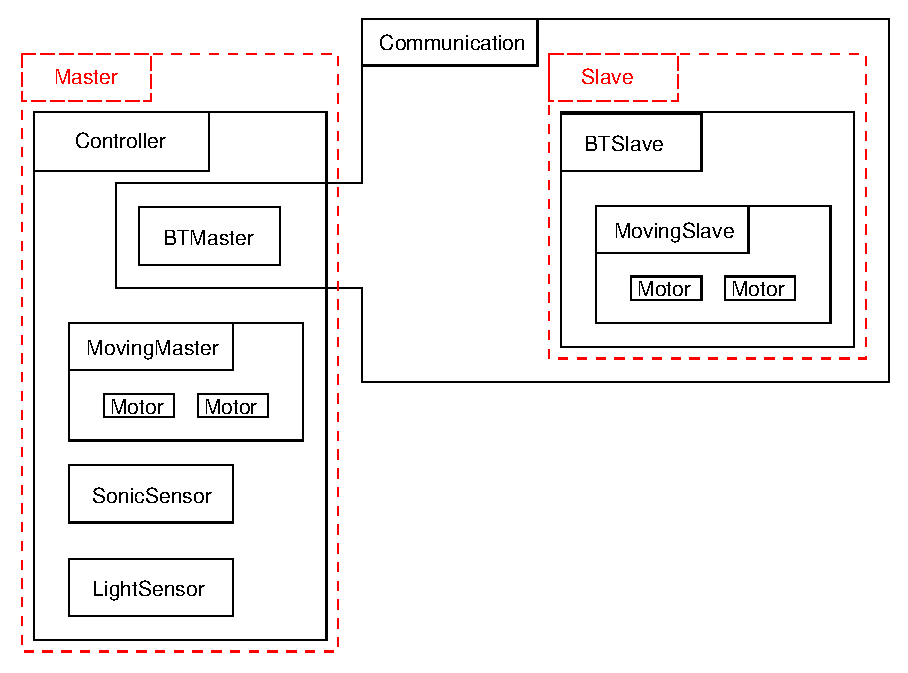
\includegraphics{ARmodel.eps}
    \caption{Architecture AltaRica}
   \end{center}
  \end{figure}

  \subsection{Les capteurs et moteurs}
    
   \subsubsection{Le n\oe{}ud LightSensor}

    \paragraph{\underline{Description\\}}
    Ce noeud correspond au capteur de lumière, et possède une variable 
    de flux $value$. L'action du senseur de lumière est donc véritablement 
    représentée par cette variable de flux, puisque les valeurs lues par
     le capteur sont "incontrôlables".

    \paragraph{\underline{Le source Altarica\\}}
    \verbatiminput{../src/altarica/alt/LightSensor.alt}
   
    \paragraph{\underline{La spécification\\}}
    \verbatiminput{../src/altarica/acheck/LightSensor.acheck}

    \paragraph{\underline{La sémantique\\}}
    ~\\
    \begin{figure}[!ht]
     \begin{center}
      \includegraphics{../src/altarica/LightSensor.eps}
      \caption{LightSensor}
     \end{center}
    \end{figure}

    \paragraph{\underline{Les résultats\\}}
    \verbatiminput{../src/altarica/LightSensor.prop}
    \verbatiminput{../src/altarica/LightSensor.res}
   
   \subsubsection{Le n\oe{}ud UltraSonicSensor}
   
    \paragraph{\underline{Description\\}}
    De la même manière que le noeud LightSensor, UltraSonicSensor
    comporte une variable de flux $d$ booléenne qui représente le fait
    que l'esclave soit derrière le robot maître ou pas.

    \paragraph{\underline{Le source Altarica\\}}
    \verbatiminput{../src/altarica/alt/UltraSonicSensor.alt}
    
    \paragraph{\underline{La spécification\\}}
    \verbatiminput{../src/altarica/acheck/UltraSonicSensor.acheck}
    
    \paragraph{\underline{La sémantique\\}}
    ~\\
\begin{figure}[!ht]
     \begin{center}
      
\includegraphics{../src/altarica/UltraSonicSensor.eps}
      \caption{UltraSonicSensor}
     \end{center}
    \end{figure}

    \paragraph{\underline{Les résultats\\}}
    \verbatiminput{../src/altarica/UltraSonicSensor.prop}
    \verbatiminput{../src/altarica/UltraSonicSensor.res}
   
   \subsubsection{Le n\oe{}ud Motor}
  
    \paragraph{\underline{Description\\}}
    Les moteurs sont modélisés de façon à avoir seulement trois vitesses
    possible: Avancer, stopper, reculer.

    \paragraph{\underline{Le source Altarica\\}}
    \verbatiminput{../src/altarica/alt/Motor.alt}
    
    \paragraph{\underline{La spécification\\}}
    \verbatiminput{../src/altarica/acheck/Motor.acheck}
    
    \paragraph{\underline{La sémantique\\}}
    ~\\
\begin{figure}[!ht]
     \begin{center}
      \includegraphics{../src/altarica/Motor.eps}
      \caption{Motor}
     \end{center}
    \end{figure}

    \paragraph{\underline{Les résultats\\}}
    \verbatiminput{../src/altarica/Motor.prop}
    \verbatiminput{../src/altarica/Motor.res}
   
  \subsection{Les déplacements, n\oe{uds Moving}}

    \paragraph{\underline{Description}\\}
    Les n\oe{}uds Moving sont là pour faire la synchronisation entre les deux moteurs
    munis de roues d'un robot. On différencie le moving du robot maître
    et le moving du robot esclave. Pour le maître il y a cinq ordres
    possible: avancer, 
    s'arrêter, à gauche et demi-tour. Pour l'esclave, il y a avancer,
    s'arrêter, à gauche et à droite. Il faut savoir que les
    rotations à droite et à gauche du robot sont tout le temps de 90
    degrés.

    \paragraph{\underline{Les sources Altarica\\}}
    \verbatiminput{../src/altarica/alt/MovingMaster.alt}
    \verbatiminput{../src/altarica/alt/MovingSlave.alt}
    
    \paragraph{\underline{Les spécifications\\}}
    \verbatiminput{../src/altarica/acheck/MovingMaster.acheck}
    \verbatiminput{../src/altarica/acheck/MovingSlave.acheck}
    
    \paragraph{\underline{La sémantique\\}}
    ~\\
\begin{figure}[!ht]
     \begin{center}
      \includegraphics[width=16cm]{../src/altarica/MovingMaster.eps}
      \caption{MovingMaster}
     \end{center}
    \end{figure}

    \begin{figure}[!ht]
     \begin{center}
      \includegraphics[width=16cm]{../src/altarica/MovingSlave.eps}
      \caption{MovingSlave}
     \end{center}
    \end{figure}

    \paragraph{\underline{Les résultats\\}}
    \verbatiminput{../src/altarica/MovingMaster.prop}
    \verbatiminput{../src/altarica/MovingMaster.res}
    ~\newline
    \verbatiminput{../src/altarica/MovingSlave.prop}
    \verbatiminput{../src/altarica/MovingSlave.res}
    
  \subsection{La communication}
    
   \subsubsection{Les n\oe{}uds BTMaster, BTSlave et BTMasterSlave}
    
    \paragraph{\underline{Description}\\}
    La communication bluetooth entre les deux robots est de type
    maitre/esclave, le maitre envoie simplement des ordres à executer à
    l'esclave. Le noeud BTMaster qui sera pour le robot maitre comporte
    donc simplement les quatres même ordres que le noeud moving de l'esclave. BTSlave
    sera lui pour le robot esclave, et inclus un sous noeud de type
    Moving, afin de pouvoir synchroniser les quatre ordres possibles à un
    agissement concret de ce noeud Moving. Enfin, le noeud MBTasterSlave se
    chargera de faire la synchronisation entre les ordres des noeuds
    BTMaster et BTSlave.

    \paragraph{\underline{Les sources Altarica\\}}
    \verbatiminput{../src/altarica/alt/BTMaster.alt}
    \verbatiminput{../src/altarica/alt/BTSlave.alt}
    \verbatiminput{../src/altarica/alt/BTMasterSlave.alt}
    
    \paragraph{\underline{Les spécifications\\}}
    \verbatiminput{../src/altarica/acheck/BTMaster.acheck}
    \verbatiminput{../src/altarica/acheck/BTSlave.acheck}
    \verbatiminput{../src/altarica/acheck/BTMasterSlave.acheck}

    \paragraph{\underline{La sémantique}}
    ~\\
    \begin{figure}[!ht]
     \begin{center}
      \includegraphics[width=16cm]{../src/altarica/BTMaster.eps}
      \caption{BTMaster}
     \end{center}
    \end{figure}
    \begin{figure}[!ht]
     \begin{center}
      \includegraphics[width=16cm]{../src/altarica/BTSlave.eps}
      \caption{BTSlave}
     \end{center}
    \end{figure}
    \begin{figure}[!ht]
     \begin{center}
      \includegraphics[width=16cm]{../src/altarica/BTMasterSlave.eps}
      \caption{BTMasterSlave}
     \end{center}
    \end{figure}
    \newpage
   
    \paragraph{\underline{Les résultats\\}}
    \verbatiminput{../src/altarica/BTMaster.prop}
    \verbatiminput{../src/altarica/BTMaster.res}
    \verbatiminput{../src/altarica/BTSlave.prop}
    \verbatiminput{../src/altarica/BTSlave.res}
    \verbatiminput{../src/altarica/BTMasterSlave.prop}
    \verbatiminput{../src/altarica/BTMasterSlave.res}

  \subsection{Le n\oe{}ud Controller}
   
    \paragraph{\underline{Le source Altarica\\}}
    \verbatiminput{../src/altarica/alt/Controller.alt}
    
    \paragraph{\underline{La spécification\\}}
    \verbatiminput{../src/altarica/acheck/Controller.acheck}
    
    \paragraph{\underline{La sémantique\\}}
    ~\\
\begin{figure}[!ht]
     \begin{center}
      
\includegraphics[width=16cm]{../src/altarica/Controller.eps}
      \caption{Controller}
     \end{center}
    \end{figure}

    \paragraph{\underline{Les résultats\\}}
    \verbatiminput{../src/altarica/Controller.prop}
    \verbatiminput{../src/altarica/Controller.res}

  \subsection{Interprétation}
  
  Nous avons donc modélisé tous les comportements possibles des
  robots. De cette façon, nous pouvons vérifier que des situations
  redoutées ne se dérouleront jamais.

  Nous avons ainsi vérifié les propriétés importantes, notamment la
  principale pour la mission dans le Controller qui assure qu'on ne se
  trouve jamais sur une case noire. Nous avons commenté le code des
  spécifications afin de bien comprendre.
